\documentclass{article}

\usepackage{fullpage}
\usepackage{url}
\usepackage{bbm}
\usepackage{graphicx}
\usepackage{amsmath}
\usepackage{physics}
\usepackage{mathtools}
\usepackage{bbold}
\usepackage{slashed}
\usepackage{pxfonts}
\usepackage{multicol}
\usepackage{mathptmx}
\usepackage{simplewick}
\usepackage{placeins}

\usepackage{lmodern}
\usepackage[T1]{fontenc}
\usepackage[fontsize=13.5pt]{fontsize}

\DeclareMathOperator{\erfi}{erfi}
\newcommand{\R}{\ensuremath{\mathbb{R}}}
\newcommand{\C}{\ensuremath{\mathbb{C}}}

\title{Quantum Field Theory I Excercise 3}
\author{Idan Stark}
\date{\today}

\begin{document}
\maketitle

\section{A theory of two scalar fields}
The Lagrangian for two massive interacting real scalar fields (with different masses), $\phi$ and $\sigma$, in $3 + 1$ dimensions, is
\begin{equation}
    \mathcal{L} = \frac{1}{2}(\partial_\mu \phi)^2 - \frac{1}{2}m_\phi^2 \phi^2 + \frac{1}{2}(\partial_\mu \sigma)^2 - \frac{1}{2}m_\sigma^2 \sigma^2 - \frac{\lambda}{2} \phi^2 \sigma
\end{equation}
\subsection{Momentum-space Feynman rules}
Let us draw $\phi$ propegators as solid lines and $\sigma$ propegators as  dashed lines. The rules we get then are:
\begin{itemize}
    \item Draw fully connected amputated diagrams with n vertices.
    \item For each $\phi$ propegator (solid line), add $\frac{i}{p^2 - m_\phi^2 + i\epsilon}$.
    \item For each $\sigma$ propegator (dashed line), add $\frac{i}{p^2 - m_\sigma^2 + i\epsilon}$.
    \item For each vertex add $-i\lambda (2\pi)^4 \delta(p_1 + p_2 + p_3)$.
    \item Integrate over all undetermined momenta $\int \frac{d^4p}{(2\pi)^4}$.
    \item Divide by symmetry factor.
    \item Remove the remaining $i(2\pi)^4\delta(\sum p_i)$ factor.
\end{itemize}
\subsection{Coupling constant Scaling dimension}
Since
\begin{equation}
    \left[\partial_\mu\right] = \left[m_\phi\right] = \left[m_\sigma\right] = 1
\end{equation}
And since the Lagrangian has $\left[\mathcal{L}\right] = 4$, it's clear to see that:
\begin{equation}
    \left[\phi\right] = \left[\sigma\right] = 1
\end{equation}
As well. So, the scaling dimension of the coupling constant is:
\begin{equation}
    \left[\lambda\right] = 1
\end{equation}
This makes this theory a super-renormalizable theory, where the perturbations converge in all energy ranges, but will be more accurate the higher the energy is.
\subsection{Calculating $\mathcal{M}$ for $\phi\phi \rightarrow \phi\phi$ scattering}
Up to second order in $\lambda$, there are three contributing diagrams matching this scattering, one for each of the Mandelstam variables (see figure 1). These diagrams have two vretices, one $\sigma$ propegator, and no symmetry factor ($S = 1$). This gives:
\begin{equation}
\begin{gathered}
    -\lambda^2 \int \frac{d^4q}{(2\pi)^4} (2\pi)^4 \delta(p_1 + p_2 - q)(2\pi)^4 \delta(q - p_3 - p_4) \frac{i}{q^2 - m_\sigma^2 + i\epsilon} + \\ + 
    (p_2 \leftrightarrow -p_3) + (p_2 \leftrightarrow -p_4) + O(\lambda^3) = \\ =
    -i\lambda^2 (2\pi)^4 \delta(p_1 + p_2 - p_3 - p_4)\frac{1}{(p_1 + p_2)^2 - m_\sigma^2 + i\epsilon} + \\ + 
    (p_2 \leftrightarrow -p_3) + (p_2 \leftrightarrow -p_4) + O(\lambda^3)
\end{gathered}
\end{equation}
And so
\begin{equation}
    \mathcal{M} = -\lambda^2 \left[\frac{1}{s^2 - m_\sigma^2 + i\epsilon} + \frac{1}{t^2 - m_\sigma^2 + i\epsilon} + \frac{1}{u^2 - m_\sigma^2 + i\epsilon}\right] + O(\lambda^3)
\end{equation}
\begin{figure}[!htbp]
    \centering
    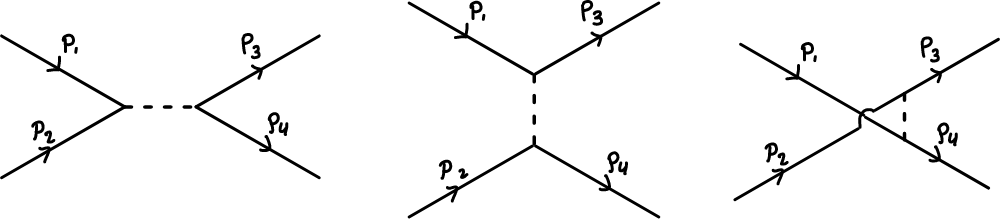
\includegraphics[width=0.5\textwidth]{figures/phiphiphiphi.png}
    \caption{The three diagrams matching the three Mandlestam variables, from right to left, $s$, $t$ and $u$. The internal propegator is a $\sigma$ propegator.}
\end{figure}
\subsection{Calculating $\mathcal{M}$ for $\phi\phi \rightarrow \sigma\sigma$ scattering}
This time, the only contributing diagrams correspond to the $t$ and $u$ channel, with the $s$ channel not applyin (see figure 2). The result is otherwise the same - 2-vertices 1-propegator diagrams, only this time the propegator is a $\phi$ propegator:
\begin{equation}
    \mathcal{M} = -\lambda^2 \left[\frac{1}{t^2 - m_\phi^2 + i\epsilon} + \frac{1}{u^2 - m_\phi^2 + i\epsilon}\right] + O(\lambda^3)
\end{equation}
\begin{figure}[!htbp]
    \centering
    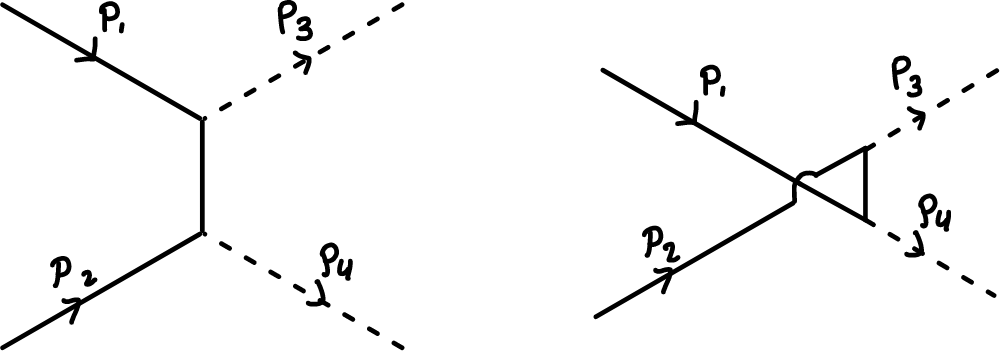
\includegraphics[width=0.5\textwidth]{figures/phiphisigmasigma.png}
    \caption{The two diagrams contributing to the $\phi\phi\rightarrow\sigma\sigma$ process.}
\end{figure}
\subsection{The $\sigma\sigma \rightarrow \sigma\sigma$ scattering}
For the $\sigma\sigma \rightarrow \sigma\sigma$ scattering to occour, at least four certices are needed. This is because any interaction of the incoming $\sigma$ fields can only result in $\phi$ fields, which must then again interact to create $\sigma$ fields. Since there is only one $\sigma$ field in each vertex, this requires one vertex for each of the incoming fields and one vertex for each of the outgoing fields. The most simple diagram accomplishing this is the four point loop diagram:
\FloatBarrier
\begin{figure}[!htbp]
    \centering
    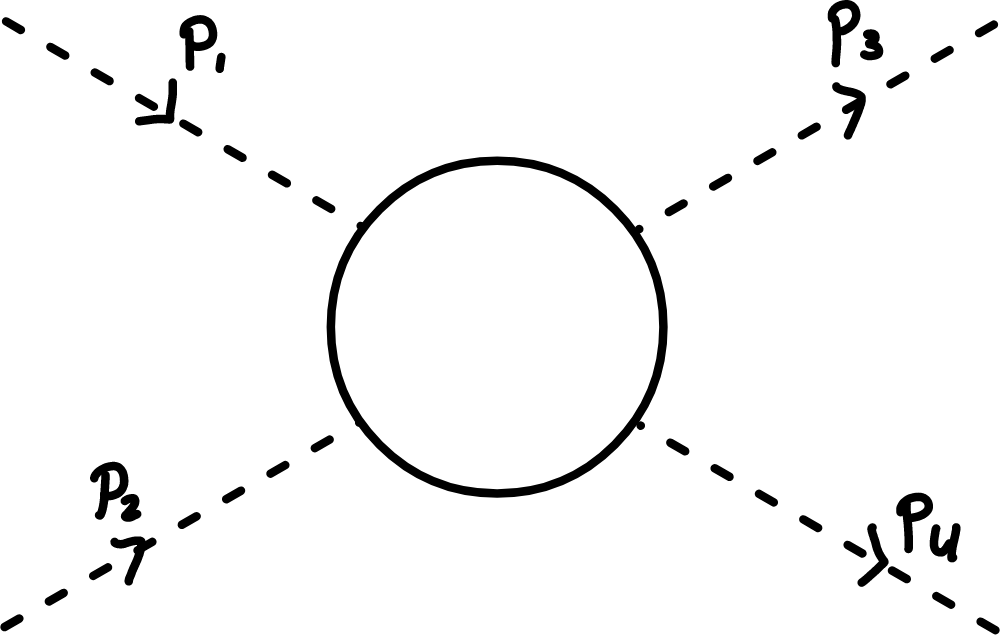
\includegraphics[width=0.5\textwidth]{figures/sigmasigmasigmasigma.png}
    \caption{The four point diagram loop for the $\sigma\sigma\rightarrow\sigma\sigma$ scattering.}
\end{figure}
\FloatBarrier
It has four vertices and four internal $\phi$ propegators, and since it has a loop that can swithc direction it has a dymmetry factor $S = 2$. This gives:
\begin{equation}
\begin{gathered}
    \lambda^4 \int \prod_{i=1}^4\frac{d^q_i}{(2\pi)^4} (2\pi)^4\delta(p_1 + q_1 - q_2)(2\pi)^4\delta(p_2 + q_2 - q_4) \times \\ \times (2\pi)^4\delta(p_3 - q_1 - p_3)(2\pi)^4\delta(q_4 - q_3 - p_4)\prod_{i=0}^4\frac{i}{q_i^2 - m_\phi^2 + i\epsilon} = \\ =
    \lambda^4 \int \frac{d^q}{(2\pi)^4} (2\pi)^4\delta(p_1 + p_2 - p_3 - p_4)\frac{1}{q^2 - m_\phi^2 + i\epsilon} 
    \times \\ \times
    \frac{1}{(q + p_1)^2 - m_\phi^2 + i\epsilon}
    \frac{1}{(q + p_3)^2 - m_\phi^2 + i\epsilon}
    \frac{1}{(q + p_3 + p_4)^2 - m_\phi^2 + i\epsilon} = \\
\end{gathered}
\end{equation}
Where we first used the $\delta$ functions to integrate three of the four $q_i$s, and got:
\begin{equation}
\begin{gathered}
    q_3 = q_1 + p_1
    \qquad
    q_4 = q_1 + p_3 + p_4
    \qquad
    q_2 = q_1 + p_3 + p_4 - p_2
    \\
    q_1 = q_1 + p_3 + p_4 - p_2 - p_1 \rightarrow p_1 + p_2 = p_3 + p_4
\end{gathered}
\end{equation}
Then, we names $q_1 = q$ and left it as a last integratin variable, noticing that $q_2 = q_1 + p_1$. And so the contribution of this diagram to the scattering amplitude is:
\begin{equation}
\begin{gathered}
    \mathcal{M} = \lambda^4 \int \frac{d^q}{(2\pi)^4}
    \frac{1}{q^2 - m_\phi^2 + i\epsilon}
    \times \\ \times
    \frac{1}{(q + p_1)^2 - m_\phi^2 + i\epsilon}
    \frac{1}{(q + p_3)^2 - m_\phi^2 + i\epsilon}
    \frac{1}{(q + p_3 + p_4)^2 - m_\phi^2 + i\epsilon}
\end{gathered}
\end{equation}
This diagram has $L = 1$ loops, and $P = 4$ internal propegators, and so the superficial degree of divergence is \begin{equation}
    D = d \cdot L - 2P = 4 \cdot 1 - 8 = -4 < 0
\end{equation}
So we got a negative superficial degree of freedom, and since there are no subdiagrams, the integral converges.
\subsection{The symmetry of the Lagrangian}
The given Lagrangian has a discrete $\mathbb{Z}_2$ symmetry
\begin{equation}
    \phi, \sigma \rightarrow -\phi, \sigma
\end{equation}
This means that for $\phi\phi \rightarrow \phi\sigma$ scattering, the initial and final states have different parity, and since the symmetry gives parity preservation, the transformation is forbidden.

\newpage
\section{Different regularizations for the Casimir force in one spatial dimension}
\subsection{An expression for the Casimir force}
Since the vaccum energy of each part of the system is:
\begin{equation}
    \bra{\Omega}H(\Delta x)\ket{\Omega} = 
    \bra{\Omega}\sum_{n=1}^\infty \omega_n(\Delta x) \left(a^\dagger_n a_n + \frac{1}{2}\right)\ket{\Omega} = \frac{1}{2}\sum_{n=1}^\infty \omega_n(\Delta x)
\end{equation}
Where
\begin{equation}
    \Delta x = \frac{\pi n}{\Delta x}
\end{equation}
This becomes:
\begin{equation}
    \bra{\Omega}H(\Delta x)\ket{\Omega} = \frac{\pi}{2\Delta x}\sum_{n=1}^\infty n
\end{equation}
The total vaccum energy of both systems is then:
\begin{equation}
\begin{gathered}
    E_{tot}(l) = \bra{\Omega}H(l)\ket{\Omega} + \bra{\Omega}H(R - l)\ket{\Omega} = \frac{\pi}{2}\left(\sum_{n=1}^\infty n\right)\left(\frac{1}{l} + \frac{1}{R - l}\right) = \\ =
    \frac{\pi}{2}\frac{R}{l(R - l)}\left(\sum_{n=1}^\infty n\right)
\end{gathered}
\end{equation}
The force is then given by the derivative with respect to $l$:
\begin{equation}
    F_c = -\frac{dE_{tot}}{dl} = \frac{\pi}{2}\frac{R(R - 2l)}{l^2(R - l)^2}\left(\sum_{n=1}^\infty n\right)
\end{equation}
Which, even taking $R \rightarrow \infty$, diverges because of the sum:
\begin{equation}
    \lim_{R \rightarrow \infty} F_c = \frac{\pi}{2l^2}\left(\sum_{n=1}^\infty n\right) \rightarrow \infty
\end{equation}
\subsection{Heat-kernel regularization}
Let us use the regularization
\begin{equation}
    \omega_n \rightarrow \omega_n \exp[-\frac{\omega_n}{\pi \Lambda}] = \frac{\pi n}{\Delta x}\exp[-\frac{n}{\Delta x \Lambda}]
\end{equation}
For some large $\Lambda$. This gives:
\begin{equation}
    E_{tot}(l) = \frac{\pi}{2}\left[
        \frac{1}{l}\left(\sum_{n=1}^\infty n e^{-n/\Lambda l}\right) +
        \frac{1}{R - l}\left(\sum_{n=1}^\infty n e^{-n/\Lambda (R - l)}\right)\right]
\end{equation}
Now, if we mark $y = \Lambda^{-1}$, we get the energy inside the box:
\begin{equation}
\begin{gathered}
    \frac{1}{l}\left(\sum_{n=1}^\infty n e^{-n/\Lambda l}\right) =
    \sum_{n=1}^\infty \frac{n}{l} e^{-ny/l} =
    -\frac{\partial}{\partial y}\sum_{n=1}^\infty e^{-ny/l} =
    -\frac{\partial}{\partial y} \frac{1}{e^{y/l} - 1} = \\ =
    -\frac{\partial}{\partial y} \left(\frac{l}{y} - \frac{1}{2} + \frac{y}{12l} - \frac{y^3}{720l^3} + \cdots\right) =
    \frac{l}{y^2} - \frac{1}{12l} + \frac{y^2}{240l^3} + \cdots = \\ =
    \frac{l}{y^2} - \frac{1}{12l} + \frac{y^2}{240l^3} + \cdots \approx
    l\Lambda^2 - \frac{1}{12l}
\end{gathered}
\end{equation}
Where the the two step we neglected all negative orders in $\Lambda$. Acting similarly on the energy for the states outside the box, we get that the total energy is:
\begin{equation}
\begin{gathered}
    E_{tot}(l) = \frac{\pi}{2}\left(l\Lambda^2 - \frac{1}{12l} + (R - l)
    \Lambda^2 - \frac{1}{12(R - l)}\right) = \\ =
    \frac{\pi}{2}\left(R\Lambda^2 - \frac{1}{12} \frac{R}{l(R - l)}\right)
\end{gathered}
\end{equation}
For large $R$, the first order contribution is $\frac{\pi}{2}R\Lambda^2$.
And the Casimir force:
\begin{equation}
    F_c = -\frac{d E_{tot}}{dl} = \frac{\pi}{24}\frac{R(2l - R)}{l^2(l - R)^2} \xrightarrow{R \rightarrow \infty} - \frac{\pi}{24l^2}
\end{equation}
\subsection{$\zeta$ function regularization}
Let us use the regularization
\begin{equation}
    \omega_n \rightarrow \omega_n \left(\frac{\omega_n}{\mu}\right)^{-s} = \left(\frac{\pi}{\Delta x}\right)^{1 - s}\mu^{s} n^{1 - s}
\end{equation}
Where we will take $s \rightarrow 0$ at the end. This gives the energy inside the box:
\begin{equation}
    \left(\frac{\pi}{l}\right)^{1 - s}\mu^{s}\left(\sum_{n=1}^\infty n^{1 - s}\right) = \left(\frac{\pi}{l}\right)^{1 - s}\mu^{s} \zeta(s - 1) \xrightarrow{s \rightarrow 0} -\frac{\pi}{12l}
\end{equation}
This gives the total energy:
\begin{equation}
    E_{tot}(l) = - \frac{\pi}{24}\frac{R}{l(R - l)}
\end{equation}
Which has the same $l$ dependency as in the Heat kernel regularization, giving the same force:
\begin{equation}
    F_c = -\frac{dE_{tot}}{dl} = - \frac{\pi}{24}\frac{R(2l - R)}{l^2(R - l)^2} \xrightarrow {R\rightarrow\infty} -\frac{\pi}{24l^2}
\end{equation}
\subsection{General regularization}
For a general regularization
\begin{equation}
    \omega_n \rightarrow \omega_n f\left(\frac{\omega_n}{\Lambda}\right)
\end{equation}
With a function $f(x)$ that has the properties
\begin{eqnarray}
    \lim_{x\rightarrow\infty} xf(x) = 0 \qquad f(0) = 1
\end{eqnarray}
The total energy becomes:
\begin{equation}
    E_{tot}(l) = \frac{\pi}{2}\left[
        \sum_{n=1}^\infty
        \frac{n}{l}f\left(\frac{\pi n}{l \Lambda}\right) +
        \sum_{n=1}^\infty
        \frac{n}{R - l}f\left(\frac{\pi n}{(R - l) \Lambda}\right)
    \right]
\end{equation}
Using the hint, let us take the large $R$ limit to approximate the second sum to an integral. Taking $x = \frac{n}{(R - l)\Lambda}$:
\begin{equation}
\begin{gathered}
    \sum_{n=1}^\infty \frac{n}{R - l}f\left(\frac{\pi n}{(R - l) \Lambda}\right) = \\ =
    \frac{\Lambda^2(R - l)}{\pi^2}\sum_{n=1}^\infty \frac{\pi n}{(R - l)\Lambda}f\left(\frac{\pi n}{(R - l) \Lambda}\right) \frac{\pi}{\Lambda(R - l)} \approx \\ \approx
    \frac{\Lambda^2(R - l)}{\pi^2}\int_{0}^\infty xf\left(x\right) dx \equiv \frac{\Lambda^2(R - l)}{\pi^2} I
\end{gathered}
\end{equation}
Where we defined $I$ as the numeric value from the intergation over $xf(x)$. Now let us turn to the first sum. We will use the Euler-Maclaurin formula for the difference between a sum from $a$ to $b$ to an integral on $[a, b]$:
\begin{equation}
\begin{gathered}
    \sum_{n=a}^{b} f(n) - \int_{a}^{b}f(x)dx = \\ =
    \frac{1}{2}\left(f(b) + f(a)\right) + 
    \frac{1}{12}\left(f'(b) - f'(a)\right) - 
    \frac{1}{30}\left(f'''(b) - f'''(a)\right) + \cdots
\end{gathered}
\end{equation}
Before we apply it, we must do a change of variables. Let us rewrite the first sum:
\begin{equation}
    \sum_{n=1}^\infty \frac{n}{l}f\left(\frac{\pi n}{l \Lambda}\right) =
    \frac{\Lambda}{\pi}\sum_{n=1}^\infty \frac{\pi n}{l\Lambda}f\left(\frac{\pi n}{l \Lambda}\right) = 
    \frac{\Lambda}{\pi}\sum_{n=1}^\infty x f\left(x\right)
\end{equation}
Where we redefined $x$ in terms of $l$ instead of $(R - l)$. Since the derivatives in the formula are based on the summation variable $n$, each derivative adds another factor of $\Lambda^{-1}$. Since there is a $\Lambda^1$ outside the sum, all derivatives of order two or higher will have negative powers of $\Lambda$, and we can ignore them. This leaves only the first two terms on the RHS:
\begin{equation}
\begin{gathered}
    \sum_{n=a}^{b} f(n) - \int_{a}^{b}f(x)dx =
    \frac{1}{2}\left(f(b) + f(a)\right) + \frac{1}{12}\left(f'(b) - f'(a)\right)
\end{gathered}
\end{equation}
Let us now define:
\begin{equation}
    g(x) = g\left(\frac{\pi n}{l\Lambda}\right), \qquad g(x) = xf(x)
\end{equation}
And derive:
\begin{equation}
    \frac{dg}{dn} = \frac{dg}{dx}\frac{dx}{dn} = \frac{\pi}{l\Lambda}\left[f(x) + xf'(x)\right]
\end{equation}
Finally, let us notice that:
\begin{equation}
\begin{gathered}
    g(0) = 0 \cdot f(0) = 0 \cdot 1 = 0 \qquad \lim_{x\rightarrow\infty} g(x) = 0
    \\
    \frac{dg}{dn}\Big|_0 = \frac{\pi}{l\Lambda}\left[f(0) + 0 \cdot f'(0)\right] = \frac{\pi}{l\Lambda}
    \\
    \lim_{x\rightarrow\infty} \frac{dg}{dn}\Big|_x =
    \lim_{x\rightarrow\infty} \frac{\pi}{l\Lambda}\left[f(x) + xf'(x)\right] =
    \frac{\pi}{l\Lambda} \lim_{x\rightarrow\infty} xf'(x) =
    \frac{\pi^2}{l^2\Lambda^2} \lim_{n\rightarrow\infty} n{}f'\left(\frac{\pi n}{l\Lambda}\right)
\end{gathered}
\end{equation}
The last term is again of order $\Lambda^{-2}$ and thus we can ignore it. Pluggin this into the above equation with $a = 0$ and $b = \infty$, and using the Jacobean $dn = \frac{\Lambda l}{\pi}$:
\begin{equation}
\begin{gathered}
    \sum_{n=1}^{\infty} g(n) - \frac{\Lambda l}{\pi}I =
    \frac{1}{2}\left(g(0) + \lim_{x\rightarrow\infty}g(x)\right) + \frac{1}{12}\left(\lim_{x\rightarrow\infty}\frac{dg}{dn}\Big|_{x} - \frac{dg}{dn}\Big|_{0}\right) = - \frac{\pi}{12l\Lambda}
\end{gathered}
\end{equation}
The total energy is then:
\begin{equation}
\begin{gathered}
     E_{tot}(l) = \frac{\pi}{2}\left[
        \sum_{n=1}^\infty
        \frac{n}{l}f\left(\frac{\pi n}{l \Lambda}\right) +
        \sum_{n=1}^\infty
        \frac{n}{R - l}f\left(\frac{\pi n}{(R - l) \Lambda}\right)
    \right] = \\ =
    \frac{\pi}{2}\left[
        \frac{\Lambda}{\pi}\left(\frac{\Lambda l}{\pi}I - \frac{\pi}{12l\Lambda}\right) +
        \frac{\Lambda^2(R - l)}{\pi^2}I
    \right] = \\ =
    - \frac{\pi}{24l} + \frac{\Lambda^2 R}{2\pi} I
\end{gathered}
\end{equation}
And the force:
\begin{equation}
    F_c = -\frac{dE_{tot}}{dl} = - \frac{\pi}{24l^2}
\end{equation}
As expected.
\end{document}